%%%%%%%%%%%%%%%%%%%%%%%%%%%%%%%%%%%%%%%%%
% Beamer Presentation
% LaTeX Template
% Version 1.0 (10/11/12)
%
% This template has been downloaded from:
% http://www.LaTeXTemplates.com
%
% License:
% CC BY-NC-SA 3.0 (http://creativecommons.org/licenses/by-nc-sa/3.0/)
%
%%%%%%%%%%%%%%%%%%%%%%%%%%%%%%%%%%%%%%%%%

%----------------------------------------------------------------------------------------
%	PACKAGES AND THEMES
%----------------------------------------------------------------------------------------

\documentclass{beamer}
\mode<presentation> {
\usetheme{Madrid}
}

\usepackage{graphicx} % Allows including images
\usepackage{booktabs} % Allows the use of \toprule, \midrule and \bottomrule in tables
\usepackage{tikz}
\usepackage{wrapfig}
\usepackage{multimedia}

\usepackage[T1]{fontenc}
\usepackage[scaled=0.85]{beramono}
\usepackage{listings}
\lstset{language=SQL,morekeywords={PREFIX,up,taxon,rdfs}}

%----------------------------------------------------------------------------------------
%	TITLE PAGE
%----------------------------------------------------------------------------------------

\title[Lydall Lab Meeting]{Modeling Heterogeneity in Microbial Population Dynamics} % The short title appears at the bottom of every slide, the full title is only on the title page

\author{Helena Herrmann} % Your name
\institute[] % Your institution as it will appear on the bottom of every slide, may be shorthand to save space
{
\textbf{MSc Computational Systems Biology \\ School of Computing Science, Newcastle University, UK \\~\\ Supervision by Dr Conor Lawless \\ Institute for Cell and Molecular Biosciences, Newcastle University, UK} \\ % Your institution for the title page
}
\date{July 25th, 2016} % Date, can be changed to a custom date

\begin{document}

\usebackgroundtemplate{%             declare it
\tikz[overlay,remember picture] \node[opacity=0.3, at=(current page.center)] {
   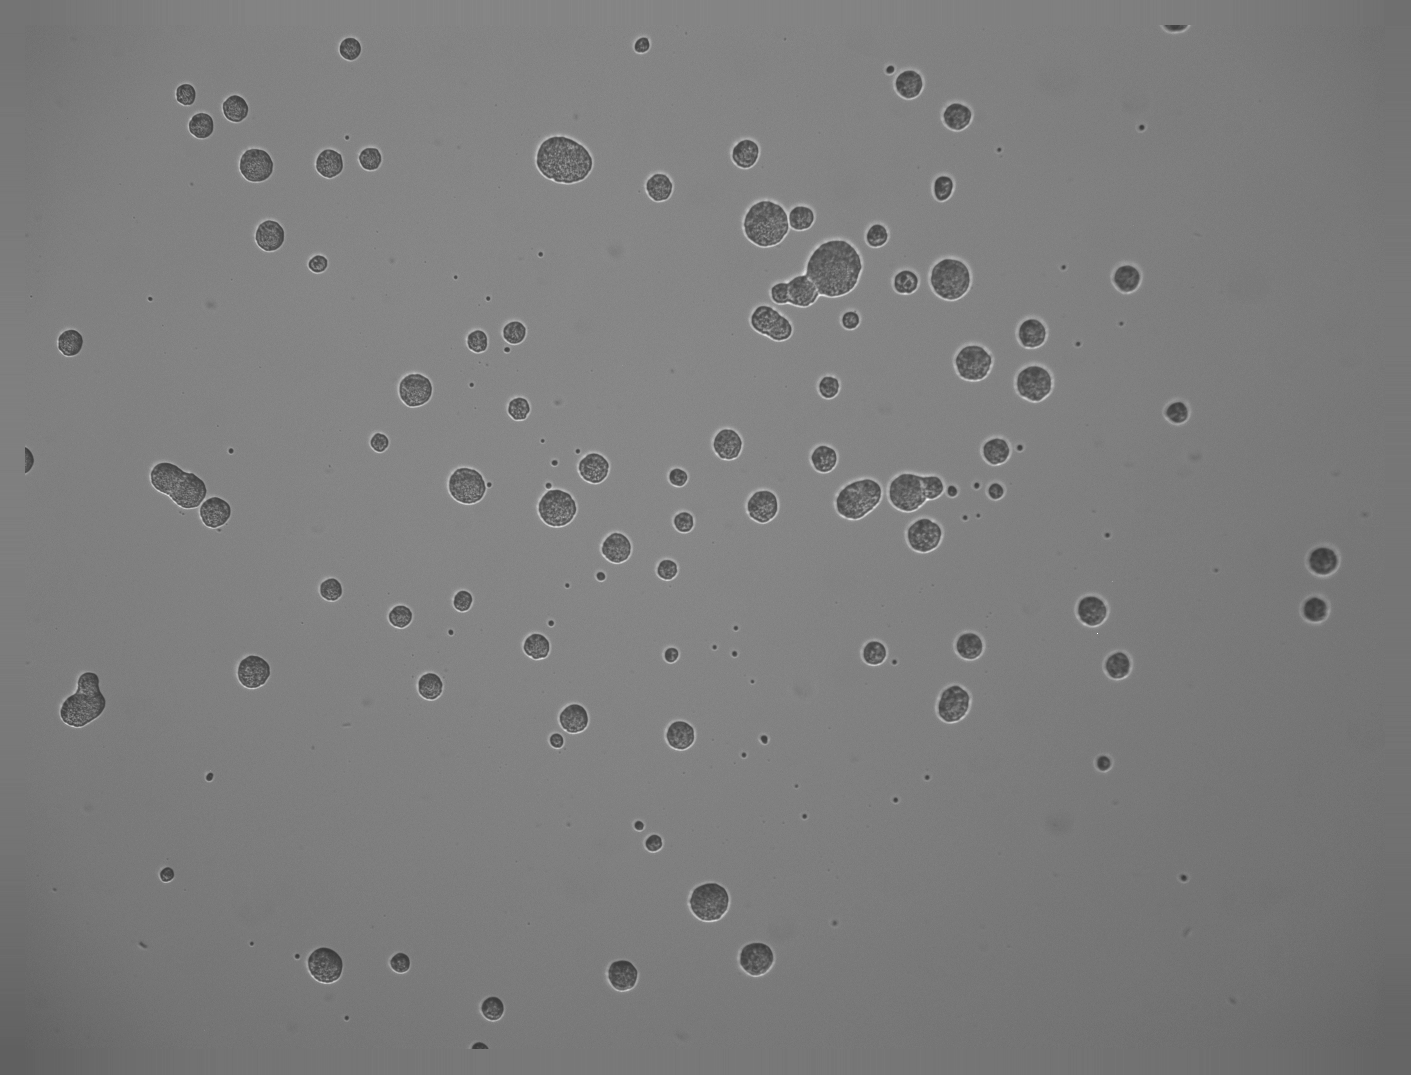
\includegraphics[height=\paperheight,width=\paperwidth]{FinishingCells.png}};
}
\begin{frame}
\titlepage % Print the title page as the first slide
\end{frame}
%\usebackgroundtemplate{ }

%----------------------------------------------------------------------------------------
%	PRESENTATION SLIDES
%----------------------------------------------------------------------------------------

\begin{frame}{movie}
\frametitle{High-Throughput Microscopy Data - $\mu$QFA}
\centering  
\begin{figure}
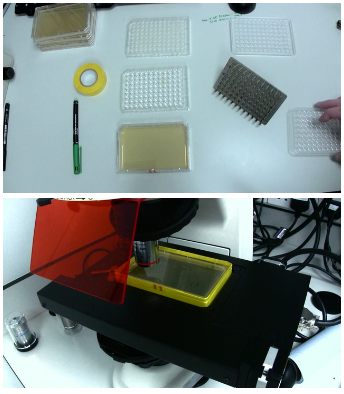
\includegraphics[width=.265\linewidth]{muQFAExp.png}
\hspace{+2em}
\movie[label=show3,width=.4\linewidth,poster
       ,autostart,showcontrols,loop] 
  {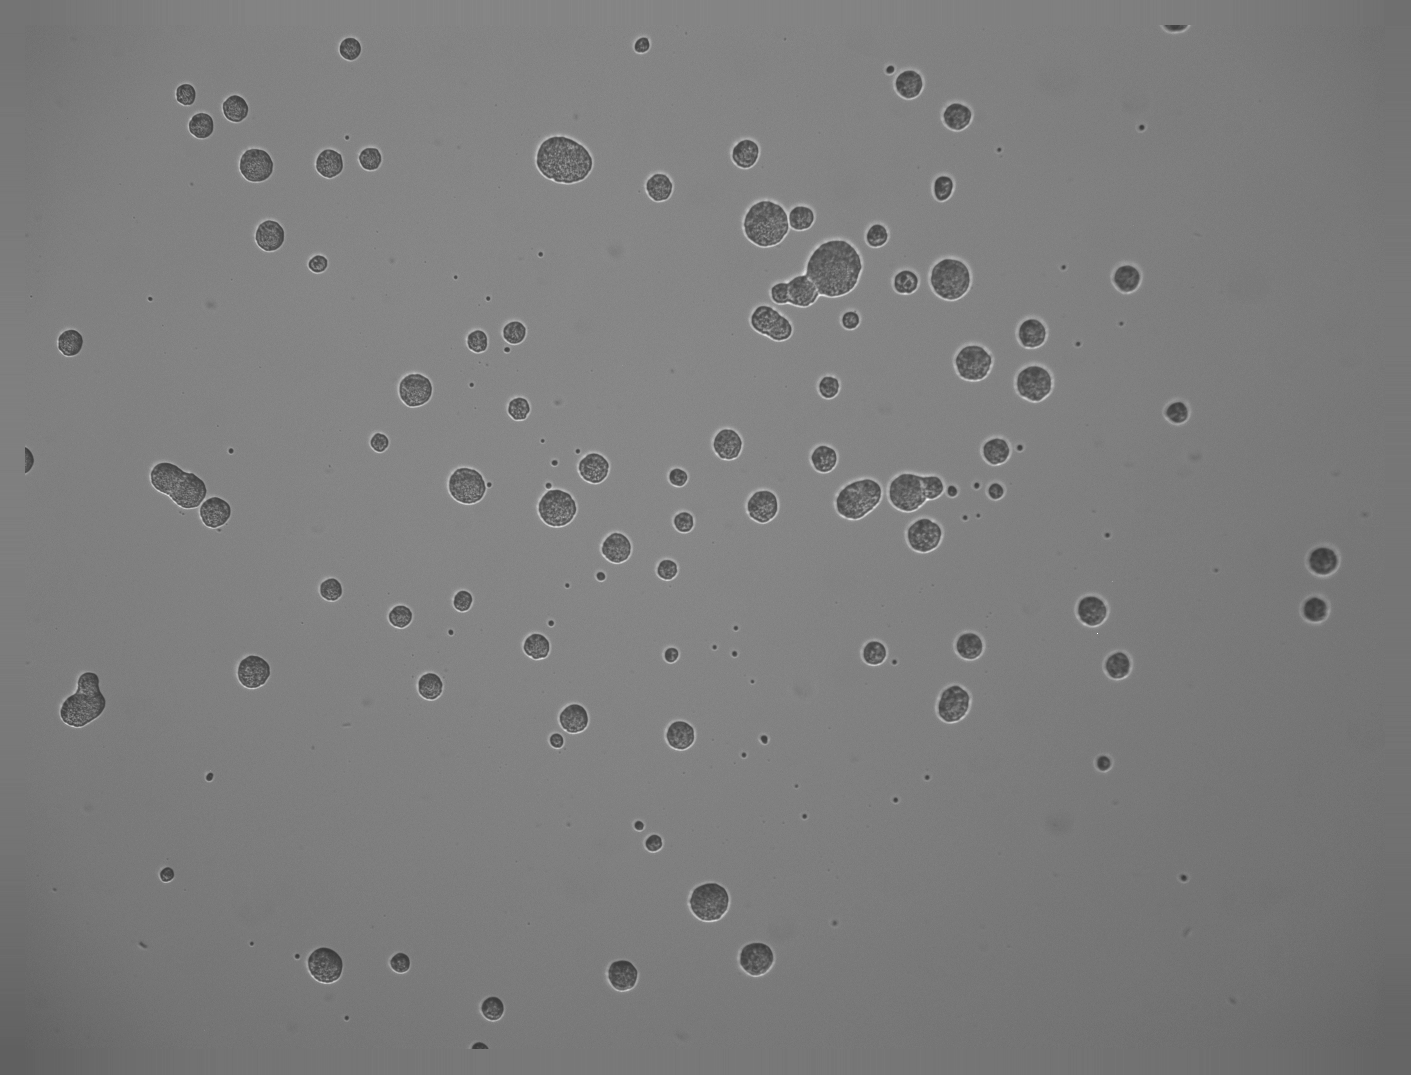
\includegraphics[width=.4\linewidth]{FinishingCells.png}}{MicroOriginal.avi}
\end{figure}
\begin{figure}
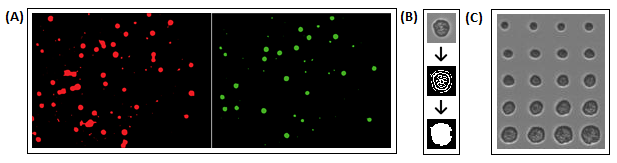
\includegraphics[width=1\linewidth]{ImageAnalysis.png}
\end{figure}
\end{frame}

% \begin{frame}
% \frametitle{$\mu$QFA - Time Courses of Clonal Colonies}
% \centering
% \begin{figure}
% 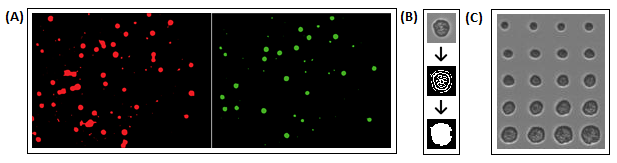
\includegraphics[width=1\linewidth]{ImageAnalysis.png}
% \end{figure}
% \vspace{-1em}
% \huge{$\downarrow$}
% \vspace{-0.2em}
% \begin{figure}
% 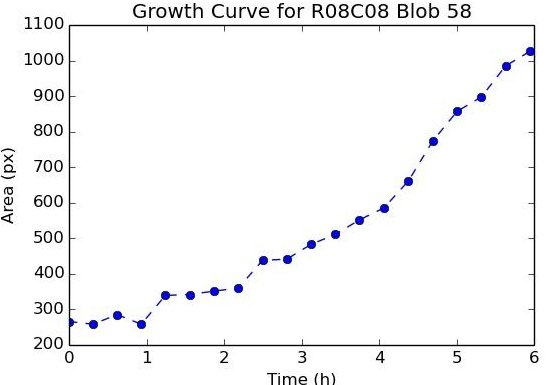
\includegraphics[width=0.4\linewidth]{FolderR08C08_Blob0058_TCGC.jpg}
% \end{figure}
% \end{frame}
% %stress the importance that this is single cell data 

\begin{frame}
\frametitle{Estimating Individual Lineage Growth Rates}
\centering
\vspace{-0.5em}
\begin{figure}
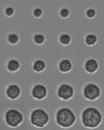
\includegraphics[width=0.08\linewidth]{FolderR08C08_Blob0014_TimeCourse.jpg}
\end{figure}
\vspace{-1em}
$\downarrow$
\vspace{-0.2em}
%\vspace{-0.5em}
% \begin{tabular}{lcr}  
%          \begin{tabular}{r}
%            \parbox{0.18 \linewidth}{%  change the parbox width as appropiate
%             \begin{center}
%             $A=A_{0}\cdot e^{r\cdot t}$
%             \end{center}}
%          \end{tabular}
%          & \begin{tabular}{c}
%            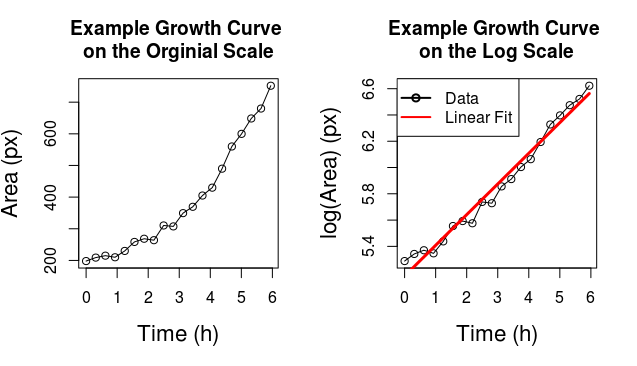
\includegraphics[width=0.4\linewidth]{ExampleGCPres.png}
%            \end{tabular}
%            %\hspace{-1em}
%           & \begin{tabular}{r}
%             \parbox{0.2\linewidth}{%  change the parbox width as appropiate
%             \begin{center}
%             $log(A)=log(A_{0})+r\cdot t$
%             \end{center}}
%          \end{tabular}  \\
% \end{tabular}
\begin{figure}
\tiny{$A=A_{0}\cdot e^{r\cdot t} \> \rightarrow \> log(A)=log(A_{0})+(r\cdot t)$ }\\
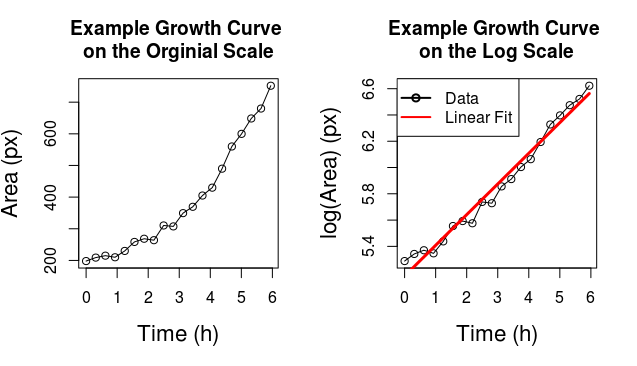
\includegraphics[width=0.45\linewidth]{ExampleGCPres.png}
\end{figure}
\vspace{-1em}
$\downarrow$
\vspace{-0.5em}
\begin{figure}
Edge peak distributions with a long right-hand tail
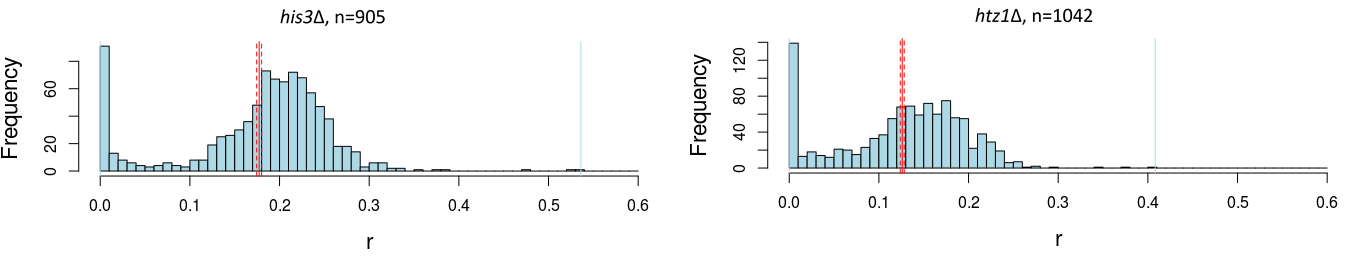
\includegraphics[width=0.9\linewidth]{GrowthRateDistr.png}
\end{figure}
%\vspace{-2em}
\end{frame}

\begin{frame}
\frametitle{Heterogeneity gives rise to an apparent lag phase.}
\begin{figure}
Population Simulations\footnote{$N_{0}=(1,...,1)$ and $n=100$}: $N(t)=\sum_{i=1}^{n}(N_{0_{i}}\cdot e^{r_{i}\cdot t})$ \\~\\
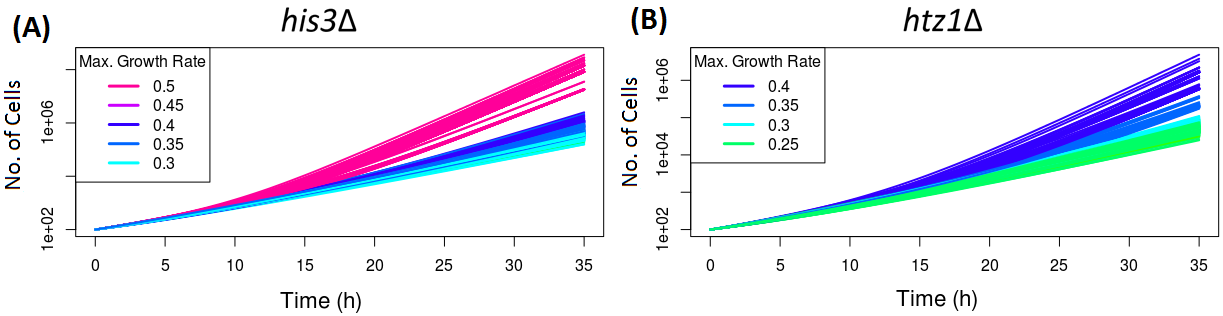
\includegraphics[width=0.8\linewidth]{PopSimCol1.png}
\end{figure}
\begin{figure}
Observed Single Lineage Growth Rates \\~\\
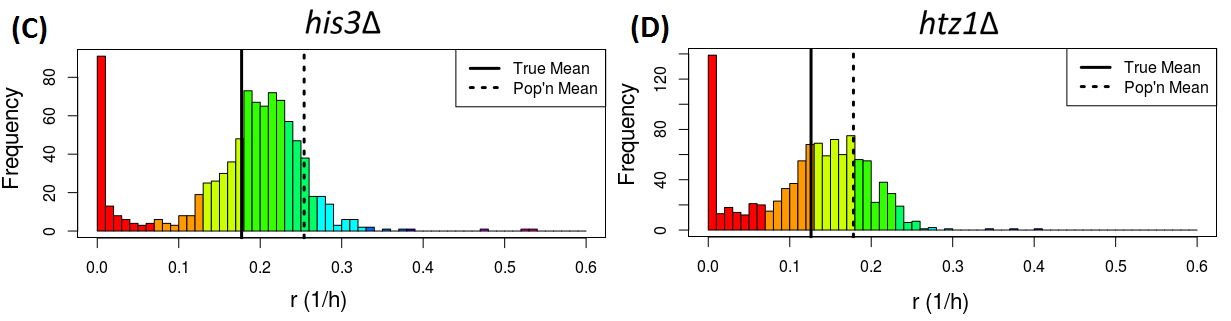
\includegraphics[width=0.8\linewidth]{PopSimCol2.png}
\end{figure}
\end{frame}

\begin{frame}
\frametitle{Population growth masks single lineage heterogeneity.}
\centering
Mixed $\rightarrow$ Clonal 
\begin{figure}
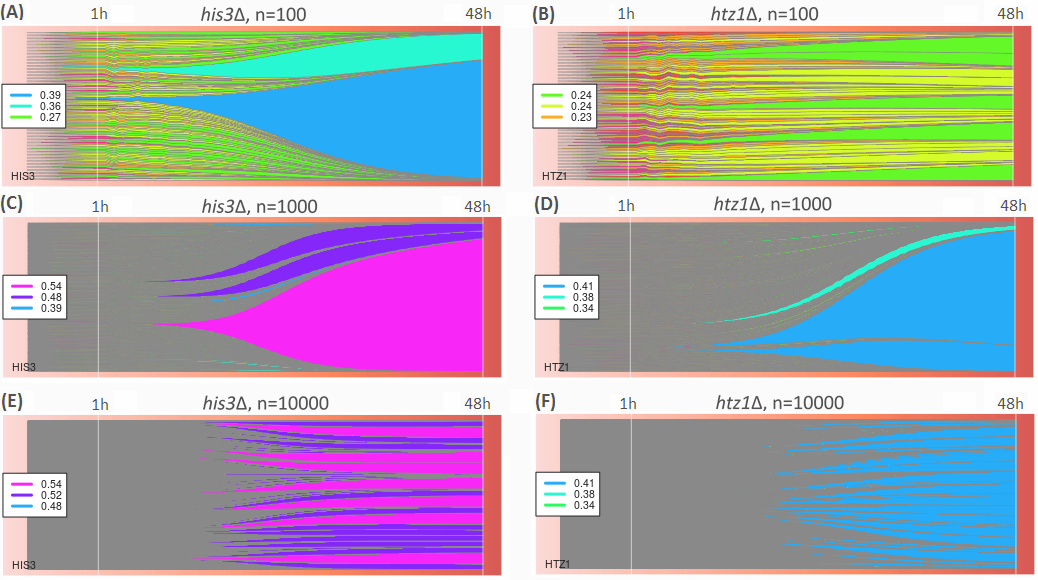
\includegraphics[width=0.9\linewidth]{FishPlot3_Names.png}
\end{figure}
\end{frame}

% \begin{frame}
% \frametitle{Fast growing lineages dominate population growth.}
% \begin{figure}
% 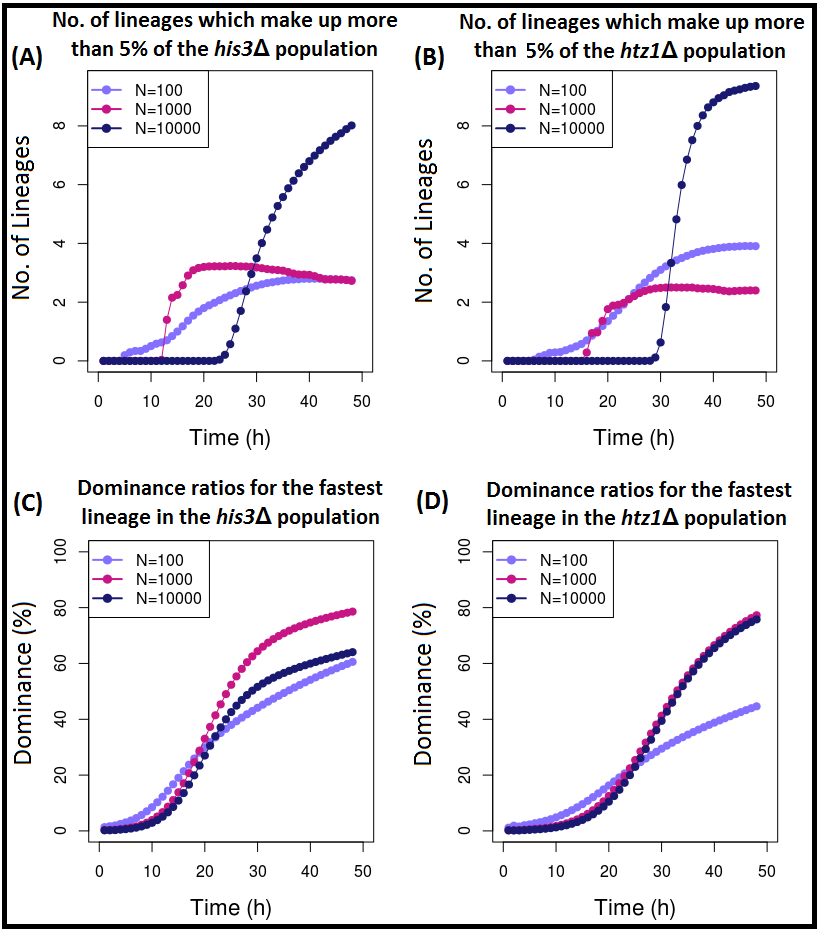
\includegraphics[width=0.55\linewidth]{Lineages5PDR.png}
% \end{figure}
% \end{frame}

\begin{frame}
\frametitle{Fast growing lineages dominate population growth.}
\centering
\begin{itemize}
\item The apparent lag phase corresponds to the time required for fast-growing lineages to dominate population growth. 
\end{itemize}
\begin{tikzpicture}
  \node (img1) {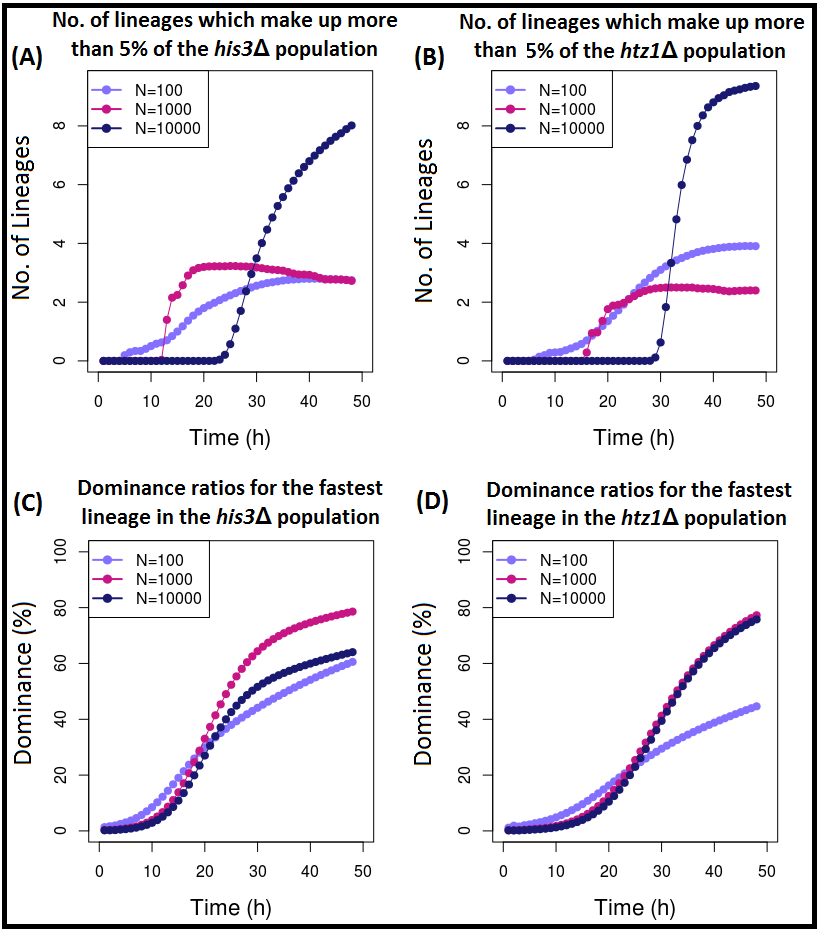
\includegraphics[width=0.45\linewidth]{Lineages5PDR.png}};
  \node (img2) at (img1.west) [xshift=-1.6cm][yshift=45]{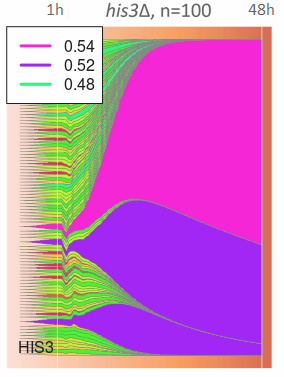
\includegraphics[height=3cm]{Pres_HIS3_FishPlot.png}};
  \node (img3) at (img1.east) [xshift=+1.8cm][yshift=-45] {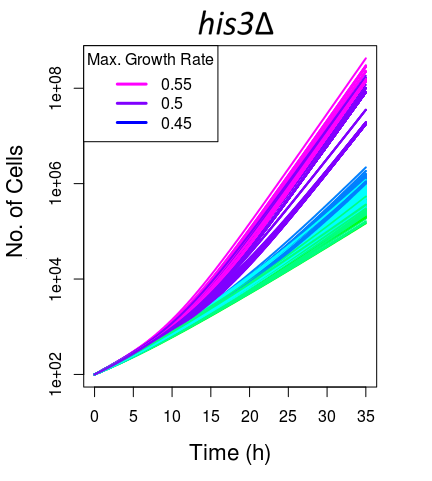
\includegraphics[height=3cm]{Pres_HIS3_ColPopSim.png}};
\end{tikzpicture}
\end{frame}

\begin{frame}
\frametitle{Experimental Design Implications}
\begin{itemize}
\item Initial population size affects apparent growth rate.
\end{itemize}
\begin{figure}
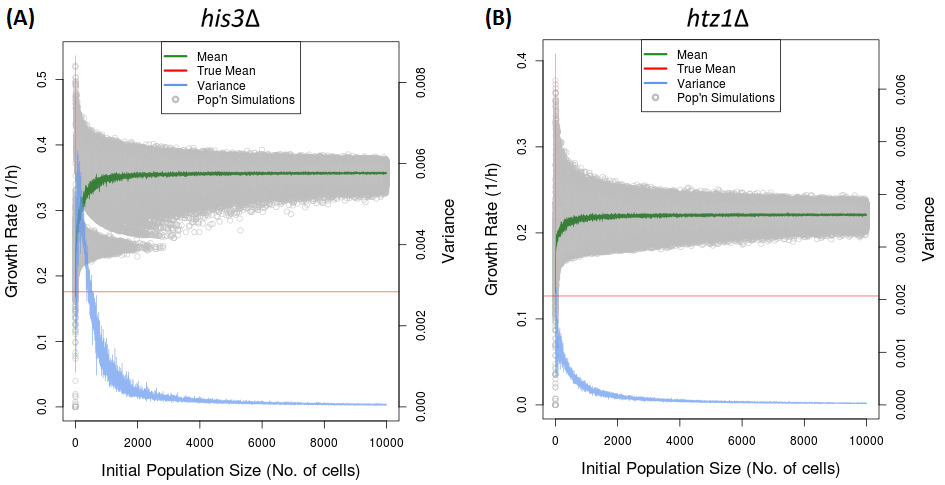
\includegraphics[width=0.95\linewidth]{InitPopSize.png}
\end{figure}
\end{frame}

% \begin{frame}
% \frametitle{Heterogeneity is important...}
% \begin{itemize}
% \item The shape of the growth rate distribution affects the extent of the apparent lag phase. 
% \item Obtaining growth rate estimates which describe the data as accurately as possible is key.
% \end{itemize}
% \begin{figure}
% 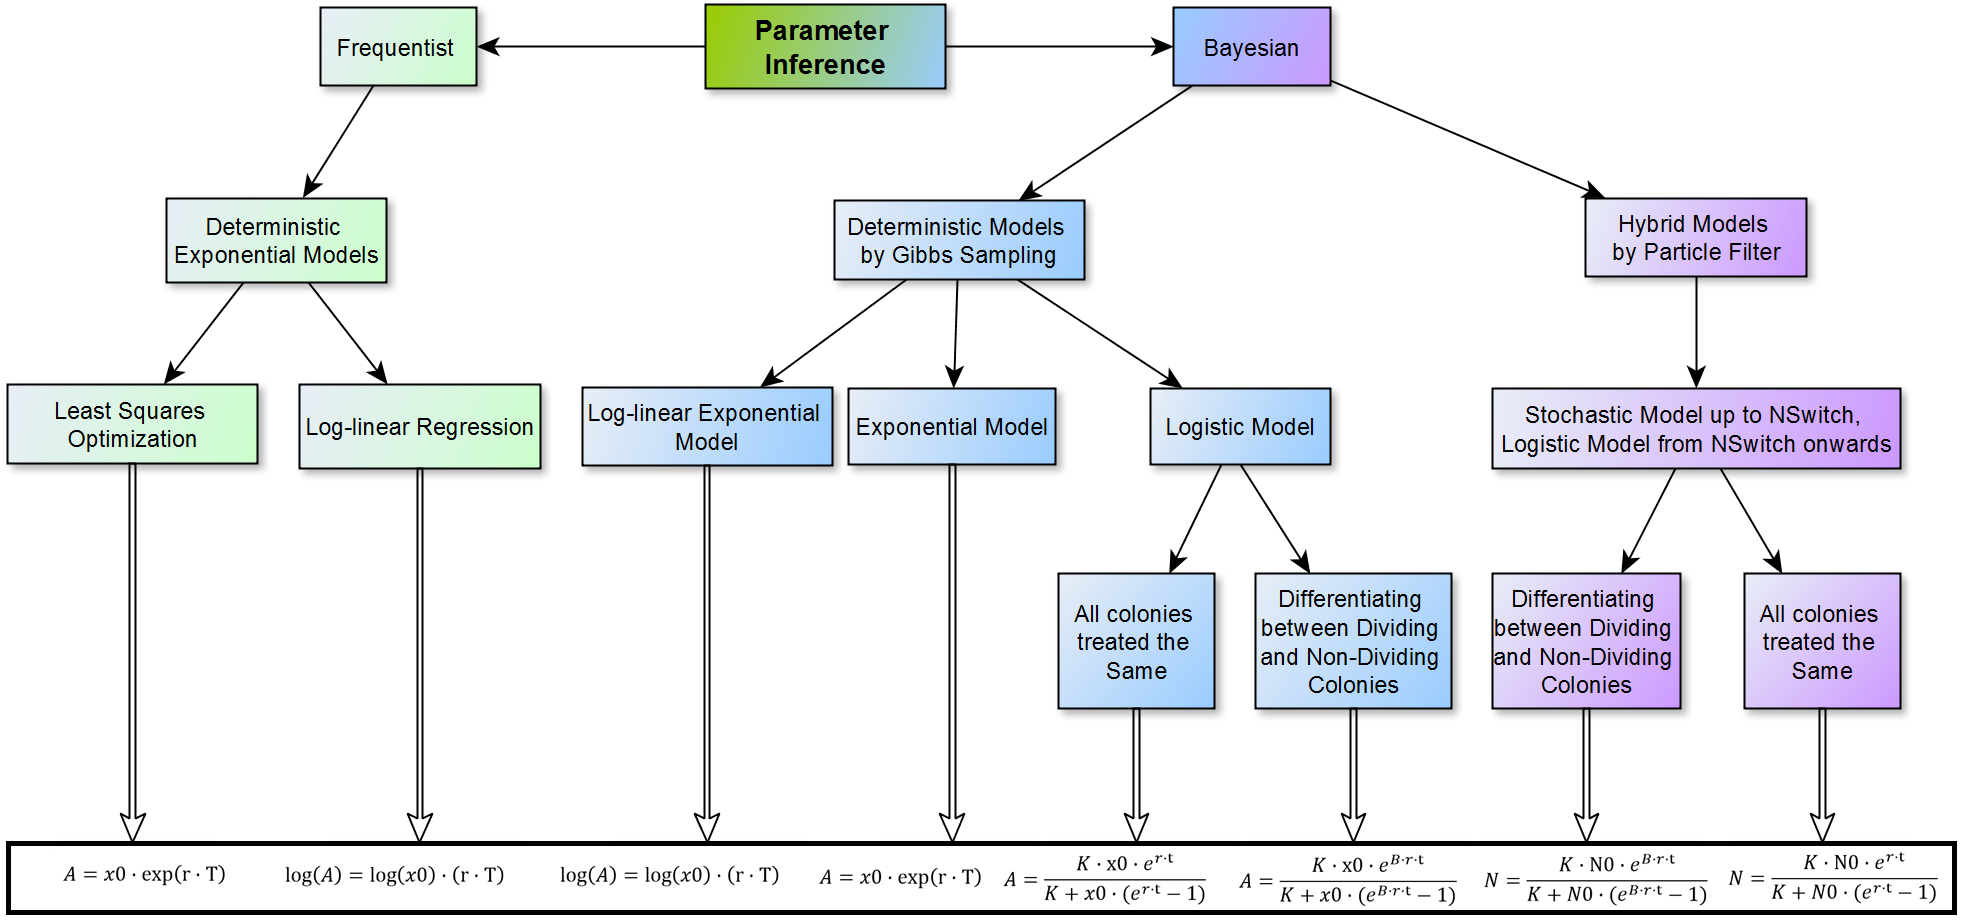
\includegraphics[width=1\linewidth]{ParInfWorkFlow.png}
% \end{figure}
% \end{frame}

\begin{frame}
%\frametitle{Any Questions?}
\centering
\Huge{Thank you}
\end{frame}


\end{document}
